\documentclass[a4paper,12pt]{article}
\usepackage[utf8]{inputenc}
\usepackage[T1]{fontenc}
\usepackage[english]{babel}
\usepackage{amsmath}
\usepackage{amssymb}
\usepackage{graphicx}
\IfFileExists{libertine.sty}{
\usepackage{libertine}
}{\typeout{> Libertine not available! Use Times instead.}
\usepackage[varg]{txfonts}}

\author{ }
\title{\vspace{-2em}
\texttt{DUMSES} \\ \textsc{Results from the test suite}}
\date{ }

%% Redefine page layout
\topmargin -65pt
\advance \topmargin by -\headheight
\advance \topmargin by -\headsep
\textheight 11.1in
\oddsidemargin 0pt
\evensidemargin \oddsidemargin
\marginparwidth 0.5in
\textwidth 6.5in

%% Change section, subsection etc. layout
\makeatletter
\renewcommand{\section}{\@startsection {section}{1}{\z@}%
             {-3.5ex \@plus -1ex \@minus -.2ex}%
             {2.3ex \@plus .2ex}%
             {\normalfont\Large\sffamily\bfseries}}

\renewcommand{\subsection}{\@startsection{subsection}{2}{\z@}%
             {-3.25ex\@plus -1ex \@minus -.2ex}%
             {1.5ex \@plus .2ex}%
             {\normalfont\large\sffamily\bfseries}}

\renewcommand{\subsubsection}{\@startsection{subsubsection}{2}{\z@}%
             {-3.25ex\@plus -1ex \@minus -.2ex}%
             {1.5ex \@plus .2ex}%
             {\normalfont\normalsize\sffamily\bfseries}}
\makeatother

\begin{document}
\maketitle

\section{Shock tube}

\begin{table}[h!]
  \begin{tabular}{c c}
    current result & reference result \\
    \multicolumn{2}{c}{$x$-direction} \\
    \includegraphics[width=.5\textwidth]{Shock_tube_x_10} &
    \includegraphics[width=.5\textwidth]{reference/Shock_tube_x_10} \\
    \multicolumn{2}{c}{$y$-direction} \\
    \includegraphics[width=.5\textwidth]{Shock_tube_y_10} &
    \includegraphics[width=.5\textwidth]{reference/Shock_tube_y_10} \\
    \multicolumn{2}{c}{$z$-direction} \\
    \includegraphics[width=.5\textwidth]{Shock_tube_z_10} &
    \includegraphics[width=.5\textwidth]{reference/Shock_tube_z_10}
  \end{tabular}
\end{table}
\clearpage

\section{Wind tunnel}

\vspace{-1em}
\begin{table}[h!]
  \begin{tabular}{c c}
    current result & reference result \\
    \multicolumn{2}{c}{$x$-direction} \\
    \includegraphics[width=.5\textwidth]{Wind_tunnel_x_10} &
    \includegraphics[width=.5\textwidth]{reference/Wind_tunnel_x_10} \\
    \multicolumn{2}{c}{$y$-direction} \\
    \includegraphics[width=.5\textwidth]{Wind_tunnel_y_10} &
    \includegraphics[width=.5\textwidth]{reference/Wind_tunnel_y_10} \\
    \multicolumn{2}{c}{$z$-direction} \\
    \includegraphics[width=.5\textwidth]{Wind_tunnel_z_10} &
    \includegraphics[width=.5\textwidth]{reference/Wind_tunnel_z_10}
  \end{tabular}
\end{table}
\clearpage

\section{Magnetic loop}

\vspace{-2em}
\begin{table}[h!]
  \begin{tabular}{c c}
    current result & reference result \\
    \multicolumn{2}{c}{$x$-direction} \\
    \includegraphics[width=.5\textwidth]{Magnetic_loop_x_10} &
    \includegraphics[width=.5\textwidth]{reference/Magnetic_loop_x_10} \\
    \multicolumn{2}{c}{$y$-direction} \\
    \includegraphics[width=.5\textwidth]{Magnetic_loop_y_10} &
    \includegraphics[width=.5\textwidth]{reference/Magnetic_loop_y_10} \\
    \multicolumn{2}{c}{$z$-direction} \\
    \includegraphics[width=.5\textwidth]{Magnetic_loop_z_10} &
    \includegraphics[width=.5\textwidth]{reference/Magnetic_loop_z_10}
  \end{tabular}
\end{table}
\clearpage

\section{Orszag Tang}

\vspace{-2em}
\begin{table}[h!]
  \begin{tabular}{c c}
    current result & reference result \\
    \multicolumn{2}{c}{$x$-direction} \\
    \includegraphics[width=.5\textwidth]{Orszag_Tang_x_10} &
    \includegraphics[width=.5\textwidth]{reference/Orszag_Tang_x_10} \\
    \multicolumn{2}{c}{$y$-direction} \\
    \includegraphics[width=.5\textwidth]{Orszag_Tang_y_10} &
    \includegraphics[width=.5\textwidth]{reference/Orszag_Tang_y_10} \\
    \multicolumn{2}{c}{$z$-direction} \\
    \includegraphics[width=.5\textwidth]{Orszag_Tang_z_10} &
    \includegraphics[width=.5\textwidth]{reference/Orszag_Tang_z_10}
  \end{tabular}
\end{table}

\section{Shearing conditions}

\vspace{-2em}
\begin{table}[h!]
  \begin{tabular}{c c}
    current result & reference result \\
    \multicolumn{2}{c}{Incompressible shearing wave} \\
    \includegraphics[width=.5\textwidth]{Incompressible_shearing_x_10} &
    \includegraphics[width=.5\textwidth]{reference/Incompressible_shearing_x_10} \\
    \multicolumn{2}{c}{Shearing wave} \\
    \includegraphics[width=.5\textwidth]{Shearing_wave_x_10} &
    \includegraphics[width=.5\textwidth]{reference/Shearing_wave_x_10} \\
    \multicolumn{2}{c}{Radial B-field} \\
    \includegraphics[width=.5\textwidth]{Radial_shearing_x_10} &
    \includegraphics[width=.5\textwidth]{reference/Radial_shearing_x_10}
  \end{tabular}
\end{table}

\section{Magnetorotational Instability}

\vspace{-2em}
\includegraphics[height=.7\textheight]{compHist_MaxReyDtMag}

\end{document}
